\section{Experimental Methods and Time Series Explanations}\label{sec:methods}
{\color{blue} EDITABLE}
% \begin{enumerate}
% \item \cmark  Experimental methods: (how we collect the %time series and what the times series areThis should be HPM %PAPI, which programs we model
%\item \cmark program descriptions and relevant citations
%\subitem \cmark description of \col
%\subitem \cmark description of \gcc
%\subitem \cmark description of \svd 
%\subitem \cmark description of svd regimes
% \end{enumerate}


\subsection{Time Series Collection {\color{blue} EDITABLE}}

The time-series data for these experiments was collected on an Intel Core\textsuperscript{\textregistered} i7-2600 running the 2.6.38-8 Linux
kernel.  This Nehalem chip has eight cores running at 3.40GHz and a cache size
of 8192 KB.  We collected performance traces of processor efficiency (IPC) during the execution of three exemplar programs---a simple microkernel(\col) and two complex programs: one from the
SPEC 2006CPU benchmark suite (\gcc), and one from LAPACK (\svd). In particular, we measured and aggregated the instructions executed per clock cycle (ipc)---a measure of processor efficiency---at 100,000-instruction intervals.  To record these measurements,
we used the {\tt libpfm4} library, via PAPI 5.2
\footnote{Performance Application Programming Interface}\cite{papi}, combined with a custom measurement infrastructure\cite{todd-phd} to stop program execution every 100,00-instructions and read the contents of the CPU's onboard hardware performance monitors (HPMs). HPMs are specialty registers who exist solely to store performance data.  For statistical validation we collected 15 performance traces from each program resulting in 45 total time series.


Obviously using a system to measure itself can cause interference--i.e, are you measuring the generating process cleanly or are you adding noise to the process?---but due diligence was put into monitoring the generating process of these time series without interfering with it in a significant way. For an in-depth explanation of this custom-measurement infrastructure as well as discussion on choice of interrupt rate see 
\cite{zach-IDA10,mytkowicz09,todd-phd}.


\subsection{The Programs: [[Maybe The generating processes]]{\color{blue} EDITABLE}}
We collect performance traces of processor efficiency (IPC) of three exemplar programs, [[If we change the title of the section, add this: which act as our generating processes]]---a simple microkernel(\col) and two complex programs: one from the
SPEC 2006CPU benchmark suite (\gcc), and one from LAPACK (\svd). In this section we provide a quick explanation of each program as well as an example performance trace (Seen in Figures \ref{fig:col-ts}-\ref{fig:svd-ts-colored}.
\subsubsection{\col {\color{blue} EDITABLE}}
\col is a simple three-line C program that repeatedly initializes the upper triangle of a  2048 X 2048 matrix in column-major order. While this is a very simple program it has been shown to produce time series with very complicated behavior. In fact, in \cite{mytkowicz09} it was shown that time series generated from this simple program can exhibit everything from periodicity to deterministic chaos.  A time series of the processor efficiency (IPC) of this program is shown in Figure \ref{fig:col-ts}.

\begin{figure}[htbp]
  \centering
    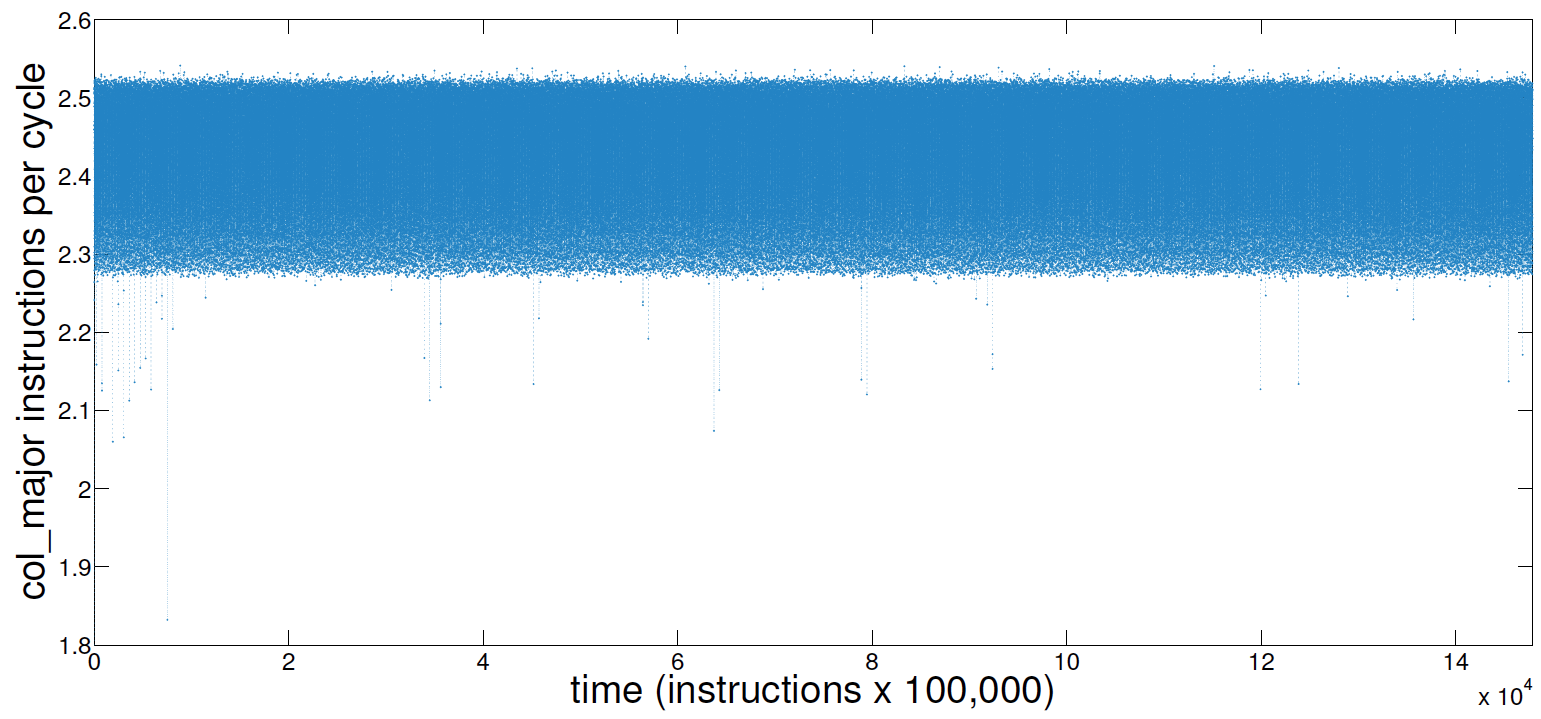
\includegraphics[width=\columnwidth]{figs/colFullTS}
    \caption{The instructions executed per CPU clock cycle (IPC) during the execution of \col. Each point is the average IPC during a 100,000 instruction period.}
    \label{fig:col-ts}
  
  \end{figure}

\subsubsection{\gcc {\color{blue} EDITABLE}}

\gcc is a benchmark program included in the SPEC CPU2006 benchmark suite \cite{spec}. This program is written by Richard Stallman and is based on Version 3.2 of {\tt gcc}. This benchmark essentially runs as a compiler with many of its optimization flags enabled, compiling a series of input files and generating x86-64 assembly code files intended for execution on AMD Opteron processors\cite{spec}. This program is more typical of programs that are used every day, as opposed to a simple micro-kernel,e.g., \col. A time series of the processor efficiency of this program running on the Intel i7-2600 is shown in Figure \ref{fig:gcc-ts}.

  \begin{figure}[t]
  \centering
    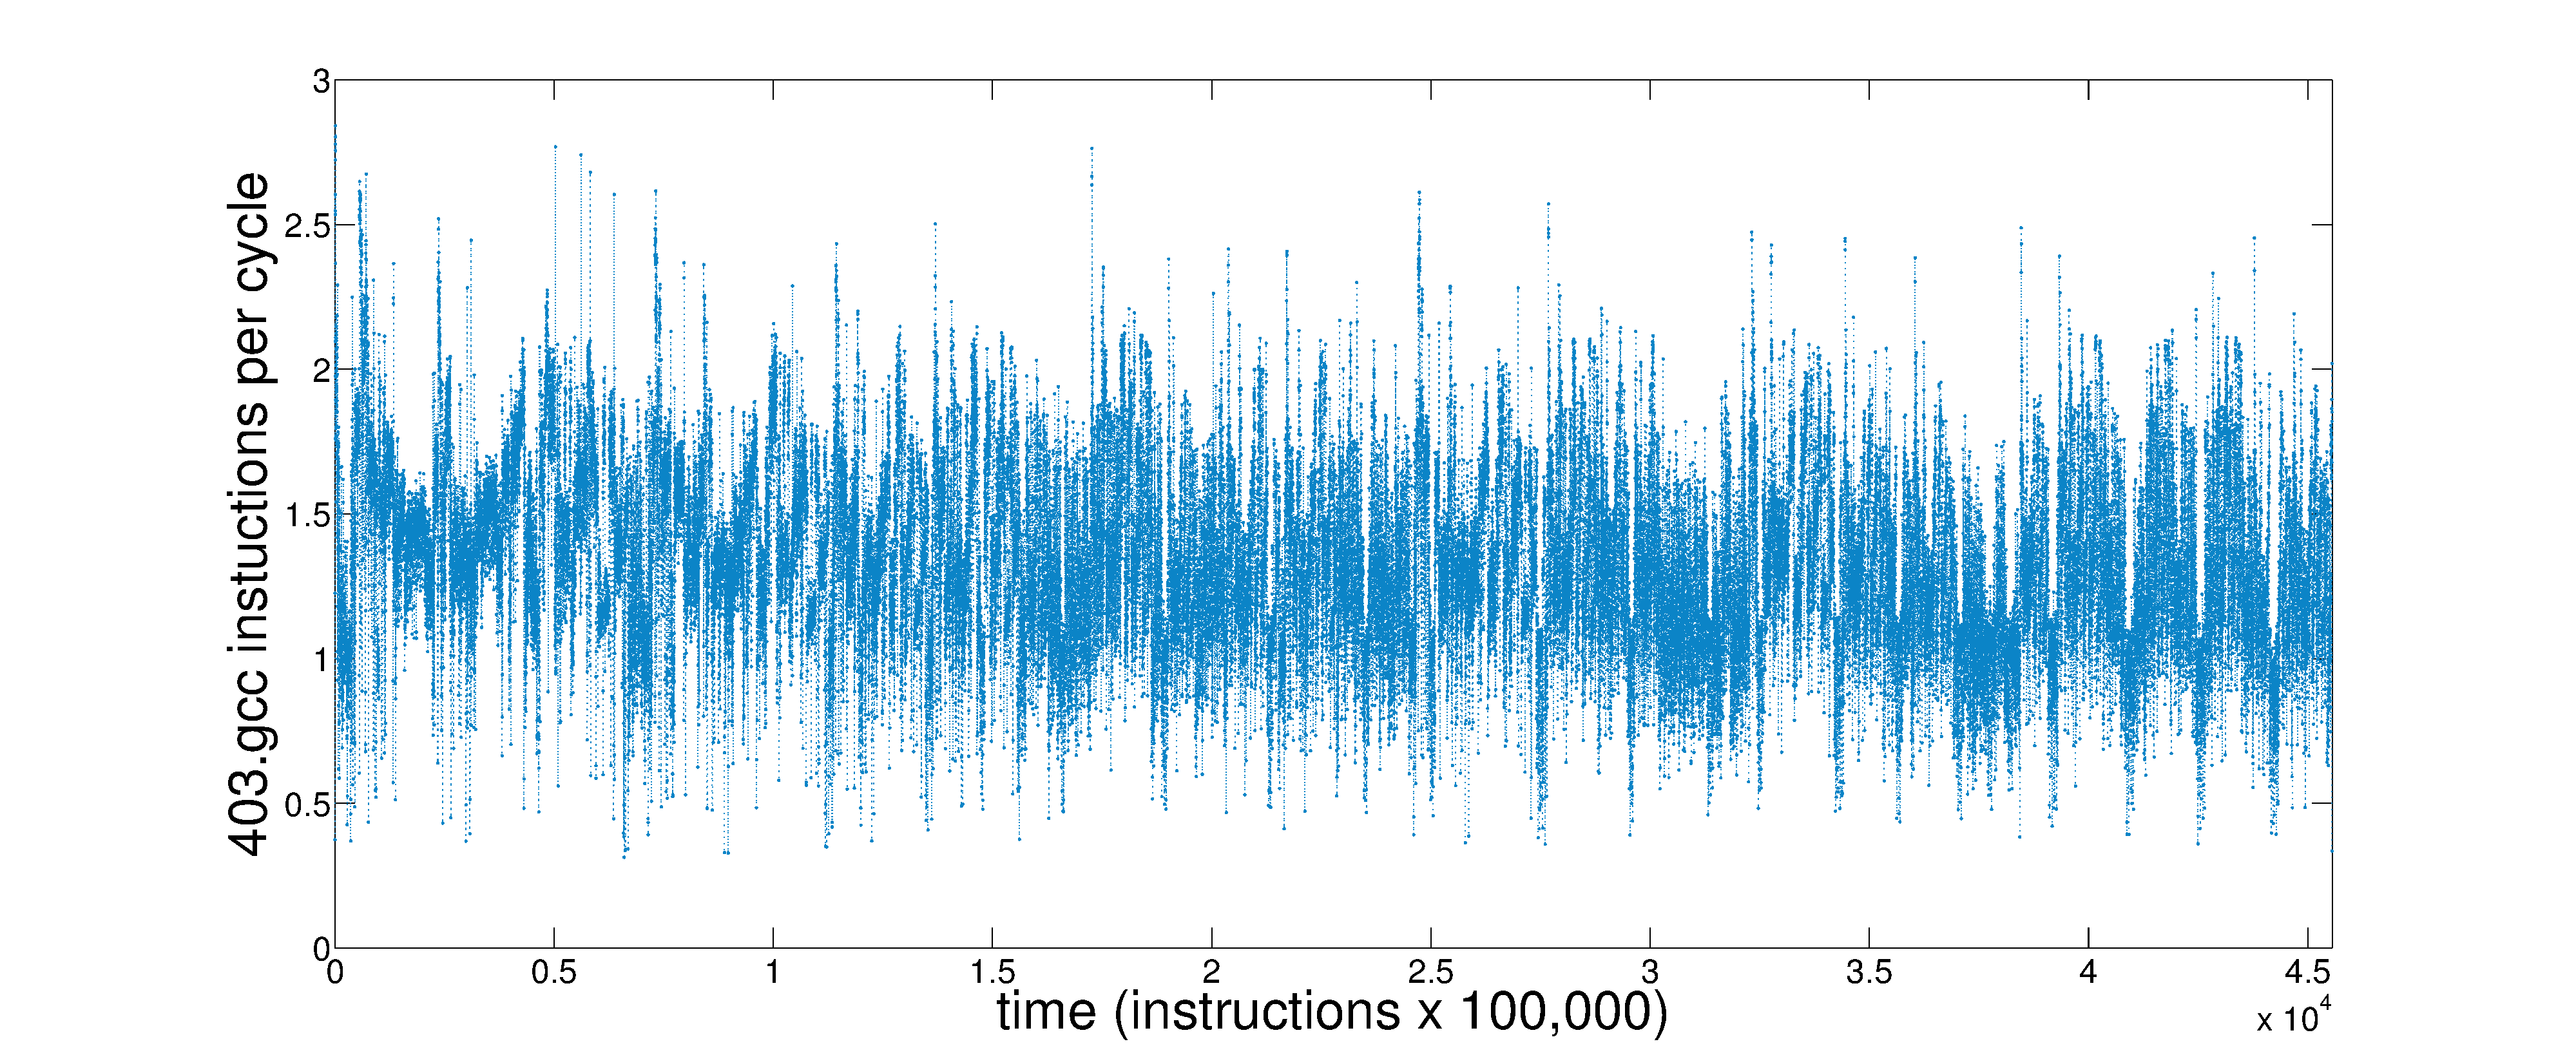
\includegraphics[width=\columnwidth]{figs/gccfullts}
    \caption{The instructions executed per CPU clock cycle (IPC) during the execution of \gcc. Each point is the average IPC during a 100,000 instruction period.}
    \label{fig:gcc-ts}
  \end{figure}

\subsubsection{\svd {\color{blue} EDITABLE}}

\svd is a Fortran program from the LAPACK suite \cite{lapack} which calculates the singular value decomposition (SVD) of a rectangular $M$ by $N$  real-valued matrix which need not contain special structure such as symmetric, positive definite etc. To execute this program we input a 750 x 1000 matrix of randomly generated entries\footnote{Multiple randomly generated matrices were investigated but no measurable effect was present in the resulting time series.}. A ``regime-colored" time series of the IPC of this program is shown in Figure \ref{fig:svd-ts-colored}. We now describe why this is done.

\begin{figure}[t]
    \centering
    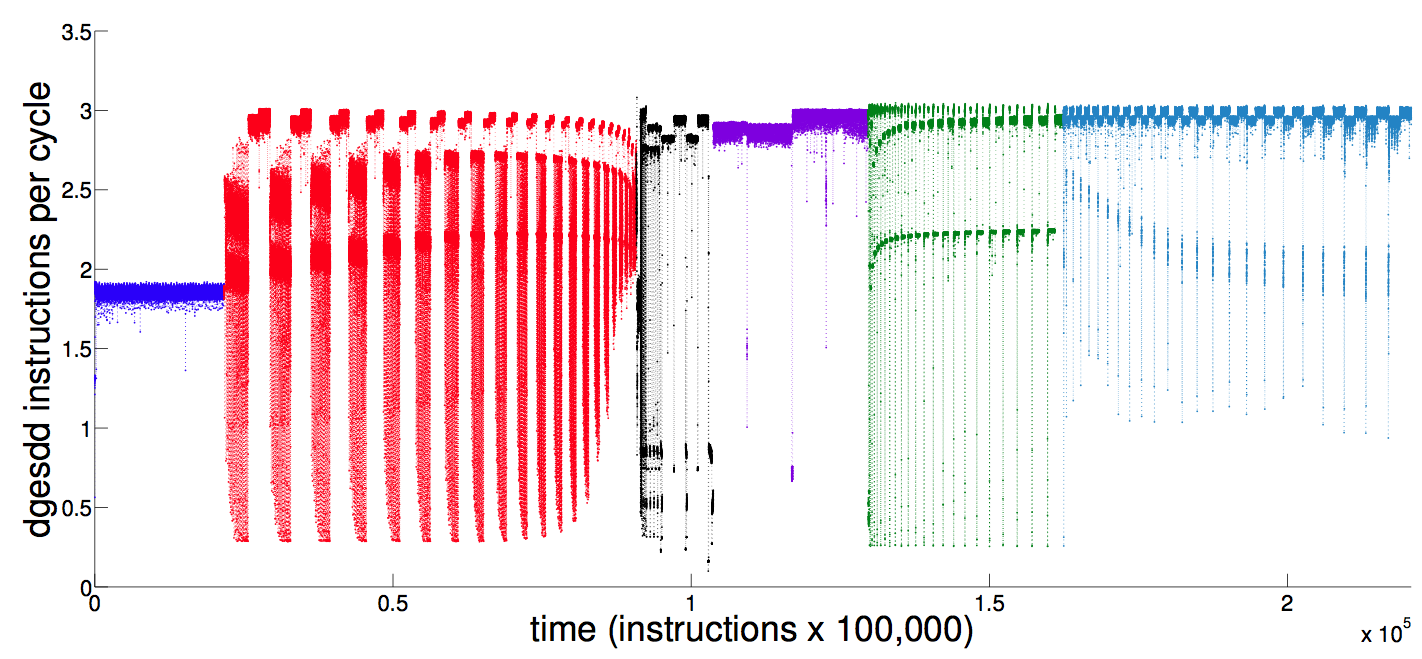
\includegraphics[width=\columnwidth]{figs/SVD1RegimesColored}
    \caption{The instructions executed per CPU clock cycle (IPC) during the execution of \svd. Each point is the average IPC during a 100,000 instruction period. The colors correspond to the six different regimes detected visually.}
    \label{fig:svd-ts-colored}
  \end{figure}

\svd brings up a very interesting point: as we observe a system the generating process can change in complexity over time. While it is clear in Figures \ref{fig:col-ts} and \ref{fig:gcc-ts} that a single system is being observed, it also appears \emph{visually} that the complexity of these two time series is consistent over time, i.e., while they are both complicated they don't appear to increase or decrease in complexity over the range of the program. \svd (seen in Figure \ref{fig:svd-ts-colored}) is different however, at least visually. Like Figures \ref{fig:col-ts} and \ref{fig:gcc-ts}, Figure \ref{fig:svd-ts-colored} is a single time series of the IPC of \svd, however as time progresses it is clear that something drastically changes in the underlying generating process and the structure of the time series  visually switches between ``regimes".

This is caused by the code of \svd moving between different subroutines as the SVD algorithm evolves, something not present in either \gcc or \col. We call these changes in \svd dynamics \emph{\svd regimes} and we have colored each of the six regimes differently in Figure \ref{fig:svd-ts-colored}. The advantage to splitting \svd into these regimes is to explore how complexity and predictability evolve over time for a system in drift. In Section \ref{sec:wpeRegime} we explore and validate the choice of these visually selected regime windows extending techniques from \cite{cao2004det}. Note, the purpose of this paper is \emph{not} to rigorously explore regime detection but to explore quantifying complexity of a time series. As such, making these regime splits serves to provide an additional 90 unique time series\footnote{Six Regimes with 15 individual runs each.} to explore. For notational convenience we refer to these time series as {\tt dgesdd$_i$} with $i \in \{1\dots6\}$ where $i$ corresponds to a regime of \svd, ordered from left to right.


For regimes \cite{cao2004det}